
\documentclass[10pt, a4paper]{article}
\usepackage[a4paper,outer=1.5cm,inner=1.5cm,top=1.75cm,bottom=1.5cm]{geometry}

%\twocolumn
\usepackage{graphicx}
\usepackage{karnaugh-map}
\usepackage{tabularx}
\usepackage{hyperref}
\usepackage[utf8]{inputenc}
\usepackage{amsmath}
\usepackage{physics}
\usepackage{amssymb}
\newcommand{\myvec}[1]{\ensuremath{\begin{pmatrix}#1\end{pmatrix}}}
\let\vec\mathbf

\begin{document}
\title{Optimization Assignment}
\author{Name:A.Gowri Priya\and Email :  \url{gowripriyaappayyagari@gmail.com}}
%\{ Wireless Communication (FWC)}
\date{}
\maketitle
  \section{Problem}
A factory makes tennis rackets and cricket bats. A tennis racket takes 1.5 hours of machine time and 3 hours of
craftman’s time in its making while a cricket bat takes 3 hour of machine time and 1 hour of craftman’s time. In a
day, the factory has the availability of not more than 42 hours of machine time and 24 hours of craftsman’s time.\\
(i) What number of rackets and bats must be made if the factory is to work at full capacity?\\
(ii) If the profit on a racket and on a bat is Rs 20 and Rs 10 respectively, find the maximum profit of the factory when
it works at full capacity.

\section{Solution}
Let's assume that
\begin{center}
Number of Tennis rackets be x\\
Number of Cricket Bats be y\\
\end{center}
\begin{tabular}{|c|c|c|c|c|}
	\hline
	\textbf{Item}&\textbf{Number}&\textbf{Machine hours}&\textbf{Craftman's hours}&\textbf{Profit}\\
	\hline
	Tennis Rackets&x&1.5&3&$Rs.20$\\
	\hline
	Cricket Bats&y&3&1&$Rs.10$\\
	\hline
	Maximum time available& &42&24\\
	\hline
\end{tabular}\\
According to question:

\begin{align}
 1.5x+3y \le 42 \\
=>3x+6y \le 84 \\
=>x+2y \le28
\end{align}
\begin{equation}
\myvec{1&2}\myvec{x\\y}\le 28
\end{equation}\\
Also,\\
\begin{align}
 3x+y \le 24 \\
\end{align}
\begin{equation}
\myvec{3&1}\myvec{x\\y}\le 24
\end{equation}\\
As we need to maximize profit,\\
Hence,function used here will be maximize Z\\
\begin{center}
profit on Tennis Racket=$Rs.20$\\
profit on Cricket Bat=$Rs.10$\\
Maximize Z=20x+10y\\
\begin{equation}
Max \;\;Z=\myvec{20&10}\myvec{x\\y}
\end{equation}\\
\end{center}
combining all constraints\\
subject to constraints\\
\begin{equation}
\myvec{1&2\\3&1}\myvec{x\\y}\le \myvec{28\\24}
\end{equation}\\
\begin{align}
  x \ge 0, y \ge 0
\end{align}
\begin{equation}
\myvec{1&2}\myvec{x\\y}\le 28
\end{equation}\\
\begin{center}
\begin{tabular}{|c|c|c|}
	\hline
	x&0&14\\
	\hline
	y&14&7\\
	\hline
\end{tabular}\\
\end{center}
\begin{equation}
\myvec{3&1}\myvec{x\\y}\le 24
\end{equation}\\
\begin{center}
\begin{tabular}{|c|c|c|}
	\hline
	x&2&8\\
	\hline
	y&18&0\\
	\hline
\end{tabular}\\
\end{center} 
\begin{center}
\begin{tabular}{|c|c|}
	\hline
	\textbf{Corner points}&\textbf{Value of Z}\\
	\hline
	(0,14)&140\\
    \hline
	(4,12)&200\\
	\hline
	(8,0)&160\\
	\hline
\end{tabular}\\

\end{center}
(i).Hence,When the factory is work at full capacity,factory produces:\\
\begin{equation}
\myvec{x\\y}=\myvec{4\\12}
\end{equation}\\
Number of Tennis Rackets=x=4\\
Number of Cricket Bats=y=12\\
(ii).Hence,Maximum profit of factory when it works at full capacity:\\
\begin{equation}
Max \;\;Z=\myvec{20&10}\myvec{x\\y}
\end{equation}\\
\begin{equation}
Max \;\;Z=\myvec{20&10}\myvec{4\\12}
\end{equation}\\
$\therefore$Maximum profit=Rs.200\\
\section{Construction}
\begin{figure}[h]
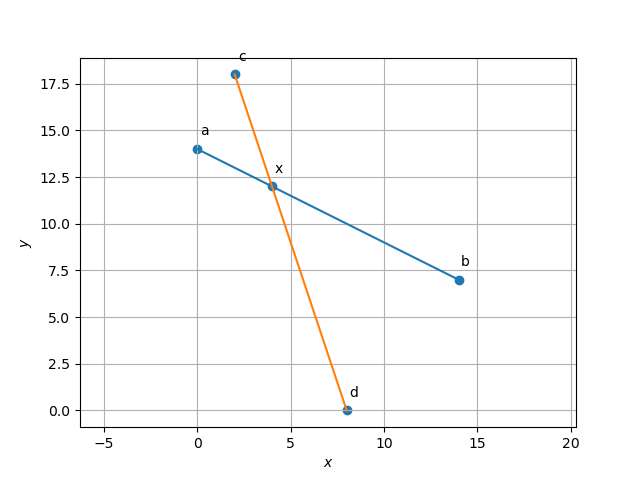
\includegraphics[scale=0.5]{optm.png} 
\end{figure}
\section{Execution}
Verify the above proofs in the following code.\\
\framebox{
\url{https://github.com/gowripriya-2002/FWC/blob/main/line_assignment/line.py}}	
\bibliographystyle{ieeetr}
\end{document}
